\chapter{Componentes de Spark}

Spark se basa en un componente principal (Core) sobre el que existen algunos componentes que extienden su uso. Los más destacables son los siguientes:\\

\textbf{Spark Core}

Como hemos adelantado en las anteriores líneas, se trata del núcleo de Spark, la base del procesamiento paralelo y distribuido. Aquí reside la funcionalidad principal de Spark para gestionar de una manera eficiente la memoria, planificar tareas, recuperarse ante fallos, entre otras posibilidades. Además, es el responsable de todas las funcionalidades de entrada y salida fundamentales. Tiene API en Scala, Java, Python y R. Los distintos componentes de Spark que presentaremos a continuación usan la lógica del Core para adaptarse a sus necesidades.\\

Es el corazón, en sentido metafórico, de Spark, pues una ventaja o desventaja en él implicará un beneficio o una pérdida en los otros módulos.  Además, en este componente se encuentra el API de las colecciones de datos RDD, concepto básico de trabajo en Spark en el que nos adentraremos en el siguiente capítulo.\\

\textbf{Spark SQL}

Spark SQL es el paquete de Spark para trabajar con datos estructurados. Permite hacer consultas distribuidas a través de SQL, así como la variante Apache Hive de SQL, llamada HiveQueryLanguage (HQL), y admite muchas fuentes de datos, incluidas tablas Hive, Parquet y JSON. Además de proporcionar una interfaz SQL para Spark, Spark SQL permite a los desarrolladores mezclar consultas SQL con manipulaciones de datos programáticos compatibles con RDD en Python, Java y Scala, todo dentro de una sola aplicación, combinando SQL con análisis complejos. Fue introducido en Spark 1.0\\

\textbf{Spark Streaming y Spark Structured Streaming}

Spark Streaming es el componente de Spark que permite el procesamiento de streams de datos. Para procesar datos en tiempo real utiliza una secuencia continua de datos de entrada. Ayuda a realizar análisis de transmisión ingiriendo datos en mini-batches, donde pueden ser procesados. Su API es muy similar a la del Sparkcore, facilitando su aprendizaje.\\

Recientemente, desde Spark 2.2, existe una nueva API de procesamiento en stream, Spark Structured Streaming. Está construida sobre el motor de Spark SQL, utiliza las API estructuradas y pretende ofrecer una mejora importante en cuanto a rendimiento y uso con respecto a su predecesor.\\

\textbf{MLlib}

Se trata de la biblioteca que contiene la funcionalidad de machine learning. Proporciona múltiples tipos de algoritmos de aprendizaje automático, así como funcionalidades de soporte tales como evaluación de modelos e importación de datos. Todos sus métodos están diseñados para escalar a través de un clúster.\\

\textbf{Graphx y GraphFrames}

Graphx es el motor de cálculos en paralelo de grafos de Spark. GraphX también proporciona varios operadores para manipular grafos (por ejemplo, subgraph y mapVertices) y una biblioteca de algoritmos de grafos comunes que veremos en los casos de uso.\\

A partir de Spark 1.4, Spark cuenta con GrapFrames, un motor nuevo  para cálculos sobre grafos. Se trata de un paquete que extiende la funcionalidad de GraphX, debido a que esta  usa DataFrames en lugar de RDD, por lo que aprovecha la optimización de estos, además de extender los lenguajes con los que puede ser usado (Scala, Java y Python).\\

\textbf{Gestor de recursos}

Spark está diseñado para escalar en un clúster, y de manera eficiente, de uno a muchos miles de nodos. Spark admite tres administradores de clústeres distintos: Hadoop YARN, Apache Mesos y StandaloneCluster Manager, lo que maximiza su flexibilidad. \\

\begin{figure}[H]
	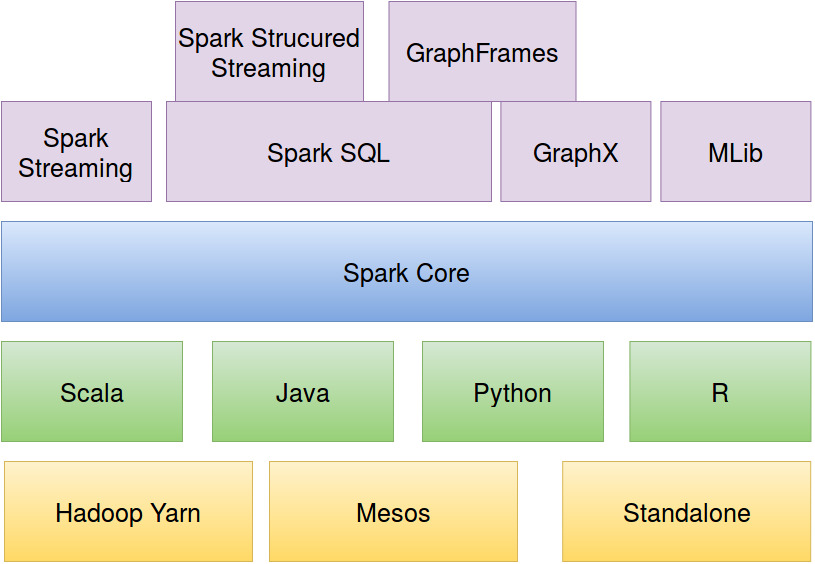
\includegraphics[scale=0.6]{img/componentes}
	\caption{Ecosistema de Spark}
	\label{Ecosistema}
\end{figure}

\section{Spark shell}
Se trata de una consola de lenguaje interactiva con la que poder trabajar de una manera rápida y sencilla con Spark. Está disponible en Scala y Python.\\

\section{Spark UI}
Es una interfaz web con la que podemos monitorizar nuestras aplicaciones en Spark.\\

\vspace*{3.5\baselineskip}
Gracias a todo este ecosistema de librerías y aplicaciones podemos considerar a Spark como una compleja y completa herramienta con la que podemos trabajar en campos muy diversos dentro del Big Data, ofreciendo además versatilidad a la hora de elegir el lenguaje con el que hacerlo.